\documentclass{article}
\usepackage[top=2.5in, bottom=1in, left=1.5in, right=1in]{geometry}
\usepackage[utf8]{inputenc}
\usepackage[backend=biber]{biblatex}
\addbibresource{references.bib}
\usepackage{graphicx}
\usepackage{wrapfig}


% listings setup to match eclipse
\usepackage{listings}
\usepackage{lstcustom}

\usepackage[utf8]{inputenc}
\usepackage[T1]{fontenc}
 
% beramono or luximono give very nice ttfamily fonts
\usepackage[scaled=0.8]{beramono}
% end listings eclipse setup

\usepackage[hypertexnames=false,hidelinks]{hyperref}

\setlength{\parindent}{0pt}
\setlength{\parskip}{6pt}

\begin{document}

\renewcommand{\lstfontfamily}{\ttfamily}
\newgeometry{top=0in, bottom=0in, left=0in, right=0in}
\thispagestyle{empty}

\includegraphics{title.pdf}
\newpage
\thispagestyle{empty}
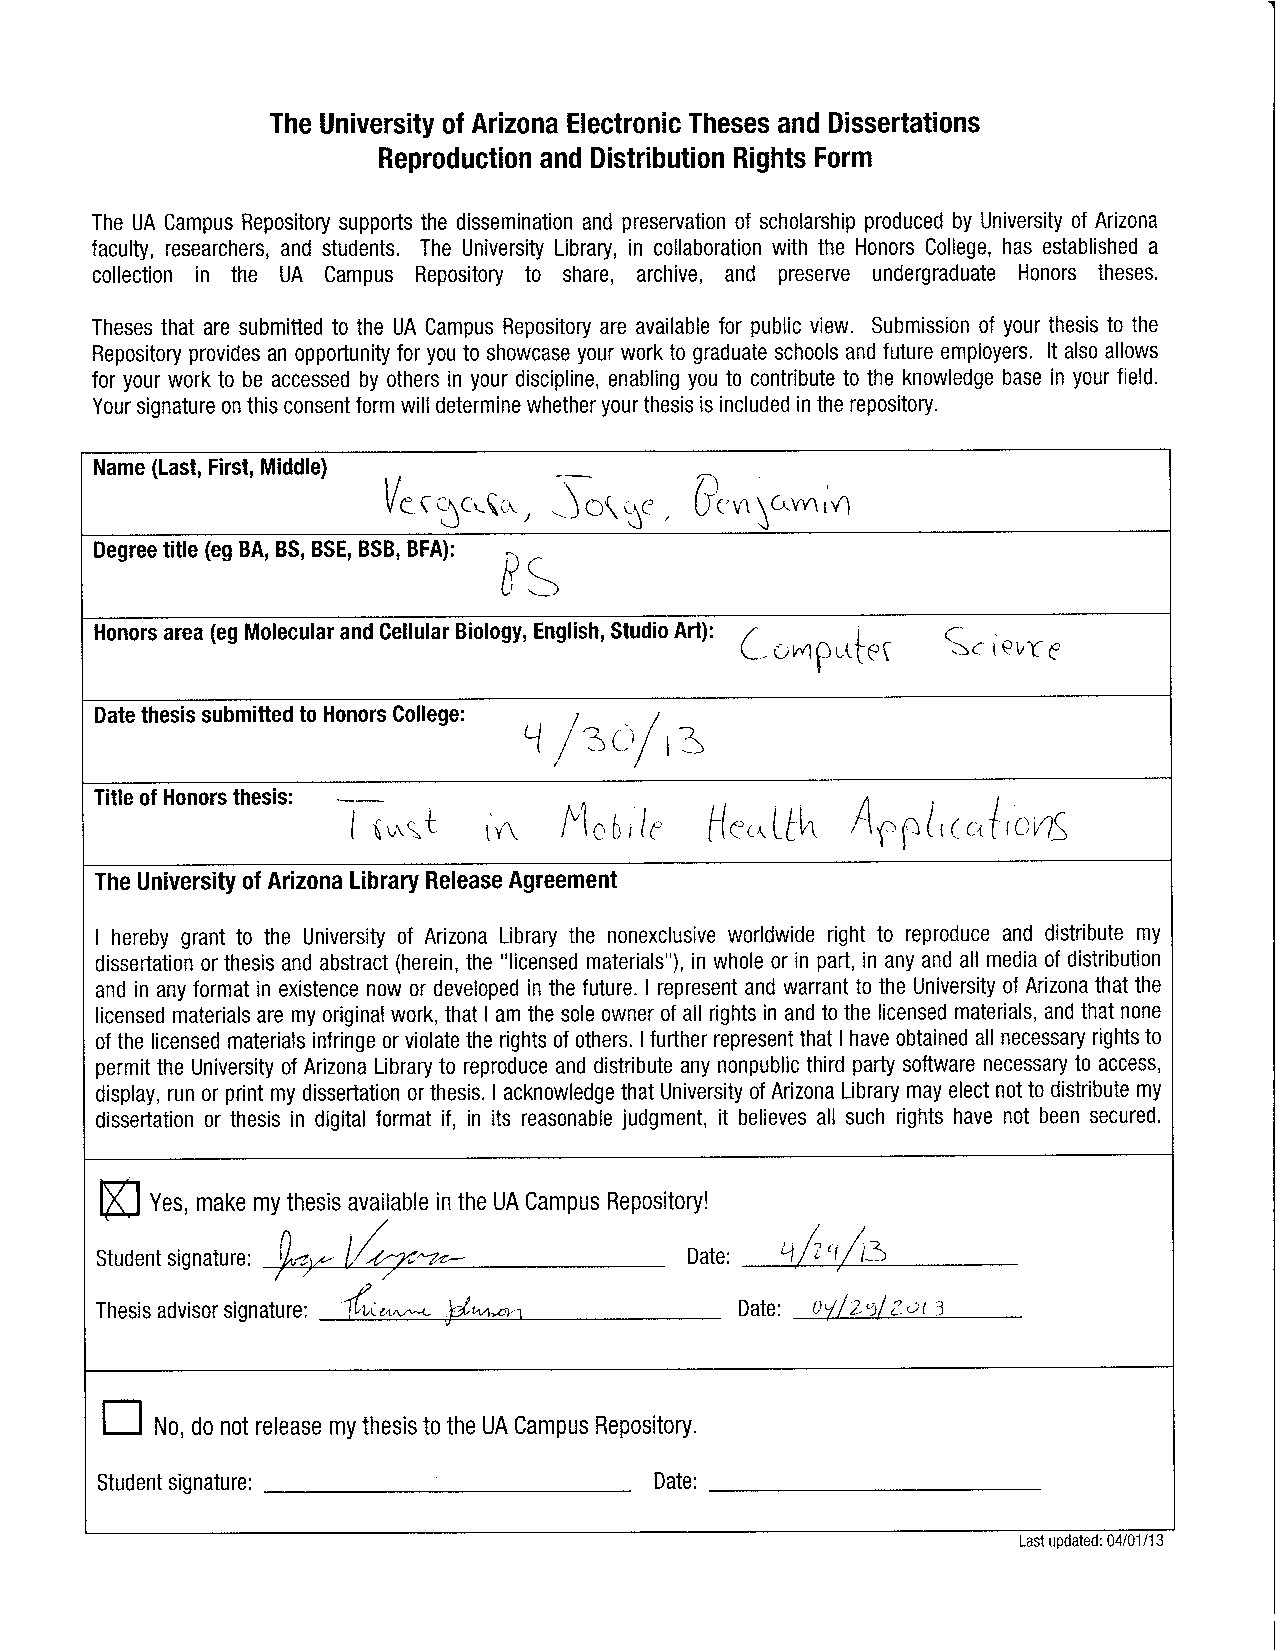
\includegraphics{release.pdf}
\newpage
\newgeometry{top=1.25in, bottom=1.25in, left=1.25in, right=1.25in}
\pagenumbering{roman}
\section*{Abstract}
As mobile devices become more prevalent in healthcare scenarios, it is becoming necessary to develop infrastructure to allow these devices to securely participate in emergency healthcare response scenarios. In this work, the scenario of an emergency response team requesting access to the health care records of a patient is analyzed. As these records may not be immediately available to the requesting party, several parties may need to be contacted to ensure to validate the identity of the requester and deliver the records.

Existing works exploring this topic are briefly analyzed. Using recommendations found in these works as well as standard technologies such as SSL, X.509, and AES, a proposed protocol for such a scenario is presented. The construction of a prototype using Android as the mobile phone OS and Tomcat as the Java HTTP Servlet container and web server is discussed, focusing on the implementation decisions as well as the difficulties encountered during development.

Finally, weaknesses of the proposed protocol that were realized during prototype implementation are discussed and future improvements are proposed. 
\newpage
\tableofcontents
\newpage
\setcounter{page}{1}
\pagenumbering{arabic}
\section{Introduction}
Mobile health is quickly emerging as an important topic in Computer Science. As mobile phones become increasingly powerful and prominent in everyday life, their potential to be used to improve healthcare outside of the hospital also increases. Oftentimes, an emergency response team needs access to the healthcare records of a patient in order to better provide care to that individual. To further complicate this problem, the patient's records may not be available at the hospital that the emergency response team belongs to. The patient may be traveling and his records may be at his home hospital in another area. This scenario is illustrated in Figure 1.

\begin{figure}[h]
\begin{center}
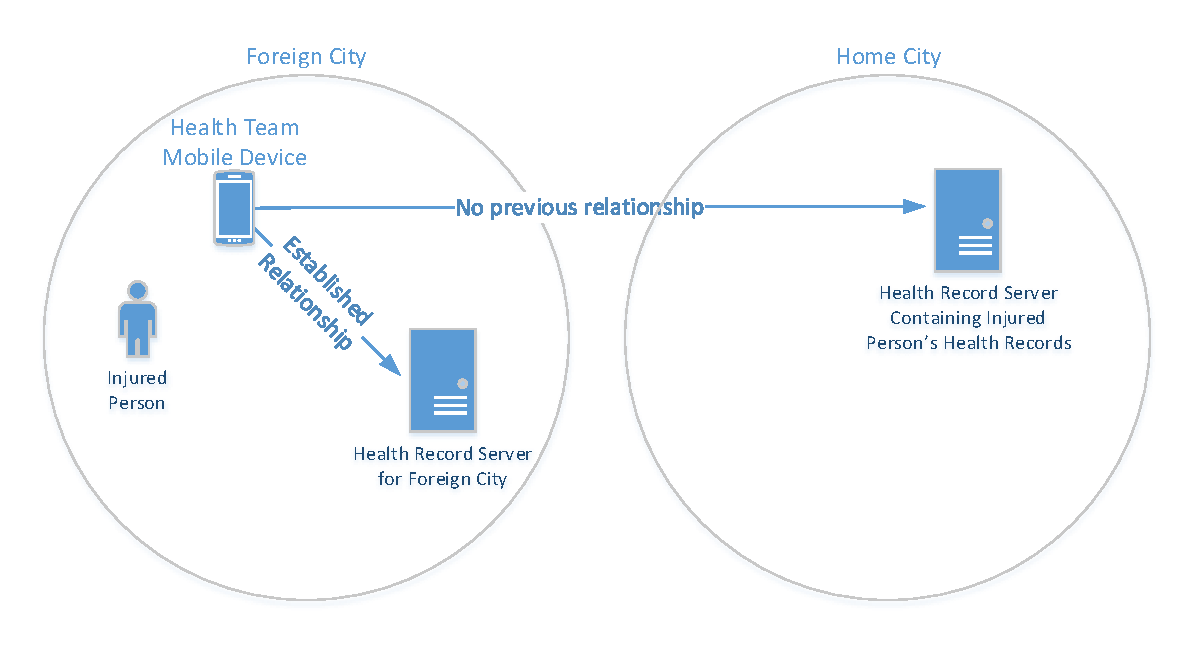
\includegraphics[scale=.75]{Drawing1.pdf}
\caption{The emergency health response team cannot access the patient's records.}
\end{center}
\end{figure}

The problem of retrieving these health records using a mobile phone does not currently have an accepted solution in use. After exploring currently proposed solutions, we attempt to combine these, as well as our own ideas, into a protocol of our creation.

In this protocol, there are two primary types of servers --- Health Record Servers and Trust Servers. Trust Servers are responsible for validating the identity of anyone that wants access to health records. These Trust Servers return an identity token which serves to confirm the trust that the Trust Servers have placed in the holder. This token can be presented to the Health Record Servers to access the needed records. The design of this protocol allows parties that may have no prior knowledge of each other to interact with some degree of trust.

Chains of trust are used utilized by the Trust Servers to deliver the identity token. A single trust server may not have the information or trust necessary to return the identity token by itself. Instead, it can contact another Trust Server that may have more ability to generate the identity token. Through this, a chain of trust is built. The first Trust Server vouches for the identity of the individual requesting the token. The second Trust Server may not know the individual, but places its trust in the first Trust Server and carries out the request. In the process of carrying out the request, the second Trust Server may have to contact additional Trust Servers, thereby lengthening the chain. This chain of trust is what allows the trusted interaction of previously unknown parties.

A prototype implementation of the protocol with several components is also constructed. The first of these components is an Android client that simulates what an emergency health care team may be using. The Android application communicates with Tomcat servers that represent several parties that interact in order to deliver the health records securely to the Android application.

This protocol was conceived after analysis of related works, which are highlighted in the following section. Section 3 discusses the design decisions and implementation process that went into the prototype. Section 4 contains conclusions drawn from the prototype development and testing, and section 5 discusses future directions for the project. Appendix A contains the code for the Android application used in the prototype, and Appendix B contains the Tomcat servlet code.
\section{Related Works}
When dealing with mobile phones, the first inclination may be to avoid servers entirely and try to construct an ad-hoc network. Research exists that uses virtual certificate authorities that allow mobile nodes to issue certificates (and thereby, confer trust) to other nodes. In such networks, link breakage becomes a concern, threatening reliability. In addition, these ad-hoc networks become quite vulnerable to attack after extended use, suggesting that at least some kind of centralized server must be used\cite{5972278}.

The problem of verifying a user's identity and trust level is a common one. In several cases this is accomplished through a capsule or token that is conferred to the requester once they are confirmed as trusted\cite{6040529}\cite{fongen1}\cite{fongen2011federated}. Encrypted usernames and passwords allow a user to access records independently of a device; however, usernames and passwords are possible to leak and must be guarded very carefully\cite{6115545}. X.509 ties identity to certificates, so information is not as accessible as with a username and a password, but is reasonably secure as long as the certificate authority is trusted\cite{4205196}\cite{6115545}\cite{5972278}\cite{fongen2011federated}.

Trust is a much more complicated subject than merely having or not having trust. Different levels of trust can also be employed to make sure that a user only has access to needed resources. Protocols exist to negotiate these different levels, as well as automatically rate the trust level of a requester. However, it is also important to remember than in a true emergency, the patient's life should always take priority over trust levels\cite{6198123}.

From these works, it is fairly clear that the main difficulty for any protocol is making sure that the trust negotiation is robust and secure. Once trust is secured by an individual, the delivery of records needs to be protected. In addition, any protocol that tries to tackle this problem on mobile phones needs to be fast and efficient enough that it can be ran on mobile smartphones.
\section{Proposed Solution}
\subsection{Identity Validation and Security}
Although many different ideas were proposed in the related works, the idea of identity tokens ended up being selected as the primary method for authentication in our prototype. The identity token system was selected primarily for its simplicity in implementation on the Android platform. Identity tokens are plain Java objects that are serialized using built in functionality of the Java libraries, and are thus easy to integrate with servers that are written in Java\cite{fongen1}\cite{fongen2011federated}.

The primary theory behind the identity tokens of being plain Java objects with short lifespans is retained in the protocol, but several other changes are made due to specific needs and challenges of our scenario. First, the identity tokens are no longer entirely public objects readable by the world. Instead, they are treated as confidential information and encrypted whenever they are sent over the network. This change was made to minimize the possibility of any security risk that may be exposed by a request for an identity token. In our scenario, a request for an identity token must be accompanied by the name (or another unique identifier) of the injured party whose health records are being sought out. This is necessary to include in the request since the requester (the medical response team) may have no prior knowledge of the injured party and cannot seek out the correct domain to request an identity token from without additional communications.

Thus, the response from the trust server must contain not only the identity token, but also information on where the health record server is that contains the requested records. The information that someone is injured or otherwise needing medical assistance is a large unintentional privacy violation if it is left unencrypted\cite{4451065}. Since this information needs to be encrypted, the encryption of the identity token does not add any complexity to the communication --- in fact, communication can be simplified, as all communication is encrypted identically. In addition, once the decision is made to encrypt the tokens, the request and response information can be included in the same Java object as the token, further simplifying the implementation of the protocol.
%\begin{wrapfigure}{r}{.35\textwidth}
%\begin{center}
%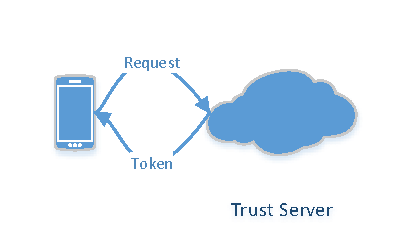
\includegraphics[scale=.75]{Drawing4.pdf}
%\caption{Request for a Token}
%\end{center}
%\end{wrapfigure}

As the identity token returned from the trust server now contains information about hospitals or health record servers that may be considered private, it is no longer wise to hand these out freely to any requester. Thus, the requesting party must verify their identity to the trust server. Table 1 reviews the properties of the identity token.

In our prototype, two-way SSL over HTTP is being used to satisfy the above needs. This handles the encryption as well as identity verification of the requester and the trust server in one step\cite{todd2003javaserver}. Correctly set up SSL should also check the revocation lists to ensure the requester has not lost their trust (for example, a certificate might be revoked after an employee no longer works at the hospital). In the prototype, Apache libraries\cite{apache} are combined with the standard Java libraries to set up the SSL connection. As SSL relies on trusted certificates distributed by a certificate authority, openSSL was used to generate and sign several certificates for all parties in the prototype\cite{manopenssl}.

\begin{center}
\begin{table}
  \begin{tabular}{ | l | l | }
    \hline
	 \multicolumn{2}{|l|}{Properties of Identity Token} \\ \hline
    userID & The userID that the requester is seeking records for. \\ \hline
    expiration & Tokens expire quickly so that they don't have to be checked for revocation. \\ \hline
    url & The URL of the Health Record Server that this token should be presented to. \\ \hline
    signature & The token is signed and hashed by the providing Trust Server. \\
    \hline
  \end{tabular}
  \caption{Properties of Identity Token}
\end{table}
\end{center}

\subsection{Trust Servers and Health Record Servers}

Of course, all the above statements rely on the existence of trust servers and health record servers that work as expected. In this case, the trust servers and health record servers were simulated by several servlets running in the Tomcat servlet container. Although these servlets were running on the same server, all communication between them was done over the network, as if they were running in separate environments.

As mentioned previously, a requester includes the name (or another more unique ID) of the individual whose health records are desired when requesting an identity token from a Trust Server. Because of the use of SSL, a Trust Server receiving a request can validate the identity of the requester. Sometimes a trust server will know exactly which health record server contains the request records, but oftentimes will have to discover this information and report it back to the requester. Ultimately, the returned product is an identity token that is signed by a Trust Server that is known to the Health Record Server holding the server. For example, if the records for ``Angela'' are held in Health Record Server A, then the requester needs to be returned an identity token signed by a Trust Server known to Health Record Server A.

Once a user has this identity token, it can then petition the Health Record Server for the records. Since the token is signed by a known Trust Server, the Health Record Server can trust that the requester has permission to access the records. The signature also ensures that the identity token was not modified. This prevents malicious users from impersonating an emergency health response team. This also prevents an emergency health response team from lying to the health record server and obtaining the records of a different person than reported to the trust server. The short expiration on the identity tokens also ensures that the requester has not had their trust revoked without having to consult a revocation list as is necessary in X.509\cite{fongen1}\cite{fongen2011federated}.

\begin{figure}[h]
\begin{center}
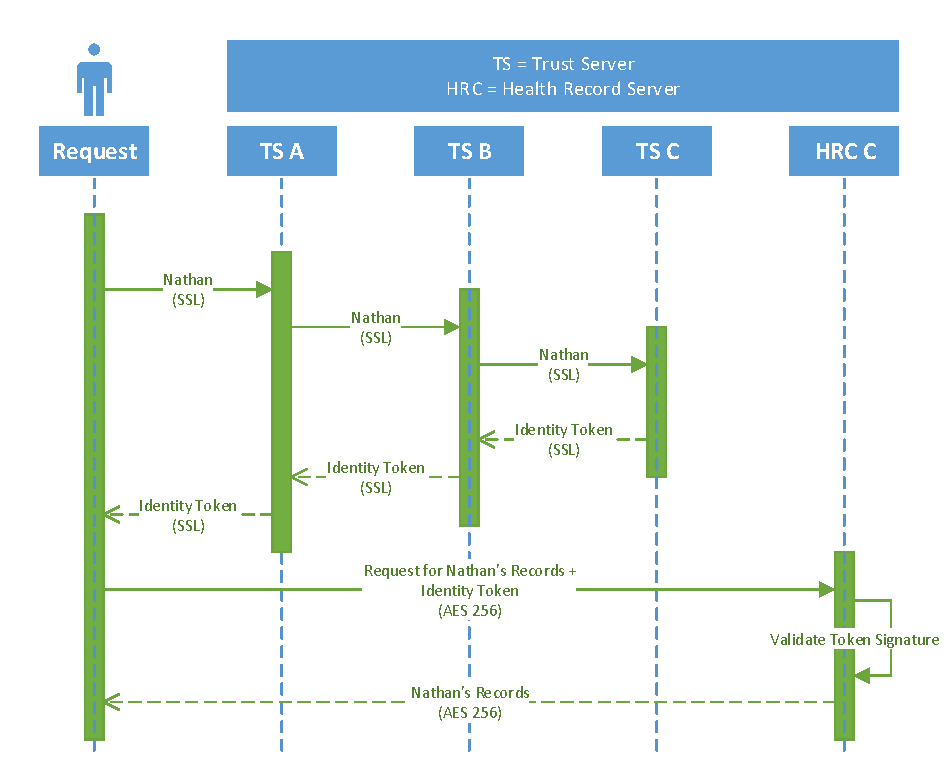
\includegraphics[scale=.75]{Drawing2.pdf}
\caption{Heath Record Retrieval Protocol}
\end{center}
\end{figure}

In the prototype, three Trust Servers and three Health Record Servers are simulated. The Trust Servers are named Trust Server A, Trust Server B, and Trust Server C. The Health Record Servers are named Health Record Server A, Health Record Server B, and Health Record C. Servers with like names are known to each other --- for example, Health Record Server A will trust identity tokens that are signed by Trust Server A. For the sake of testing, each Health Record Server contains two records. Server A contains the records of ``Angela'' and ``Rosendo''. Server B holds the records for ``Daniel'' and ``Marilyn''. Server C contains the records of ``Terry'' and ``Nathan''. Each Trust Server is aware what records their corresponding health record servers are responsible for, but does not know where any other records are held.

This means that if Trust Server A receives a request for the records of ``Nathan'', it does not know where those records are held --- only that they are not in Health Record Server A and that a token signed by Trust Server A will not be useful to the requester. Once a trust server determines that it cannot sign the token, it queries other nearby trust servers to try and retrieve the appropriately signed token for the requester. For the purposes of the prototype, Trust Server A knows of Trust Server B. Trust Server B knows of both Trust Servers A and C. Trust Server C knows only of Trust Server B. This means that a request for the health record of ``Nathan'' sent to Trust Server A will have to be forwarded to Trust Server B and finally C before a signed identity token can be returned to the requester. Since these requests are still carried out over SSL, Trust Server B is willing to trust someone trusted by Trust Server A, and so is willing to carry out its request for an identity token. In this way, a chain of trust is formed. The requester is finally returned the identity token signed by Trust Server C, as well as the URL (or other means of contact) of Health Record C, so that the requester can contact Health Record Server C directly for the records.

Upon receipt of the identity token signed by Trust Server C, Health Record Server C is then willing to send the records to the requester. As the requester and the Health Record Servers may not know each other and thus cannot use SSL, each communication should be encrypted using a symmetric key that is agreed upon beforehand. The prototype uses AES 256 to encrypt these communications. A symmetric key was chosen for the prototype as encryption using asymmetric keys is much costlier and slower. Figure 2 illustrates this entire process.

To handle most of the cryptography necessary in the prototype, the Bouncy Castle\cite{manbouncycastle} library was used to complement the built in Java functionality. Android features a version of Bouncy Castle build into the SDK, but it typically is not the latest version available. The prototype made use of some functionality only available in the newest release, but including the Bouncy Castle library in an Android project created package name conflict. To resolve this, a custom build of Bouncy Castle was created. This build simply moved everything to a unique package, as well as renamed the Bouncy Castle provider. This allowed the custom build to be registered from the Android project. As openSSL, Bouncy Castle, and Keytool (Java's bundled tool for dealing with keystores)\cite{mankeytool} operate using a variety of different formats, the open source tool Portecle\cite{manportecle} proved invaluable in converting between them.

\subsection{Performance}

The prototype seems to deliver the health records in a fairly timely fashion. Testing was done using a Motorola DRIOD 3 over a 3G connection. At the time of writing, both faster processors and faster cellular networks are fairly standard in mainstream consumer technology, so any time estimates obtained are reasonable. Figure 3 illustrates how including more Trust Server hops affected the round trip time from identity token request to identity token receipt.

\begin{figure}[h]
\begin{center}
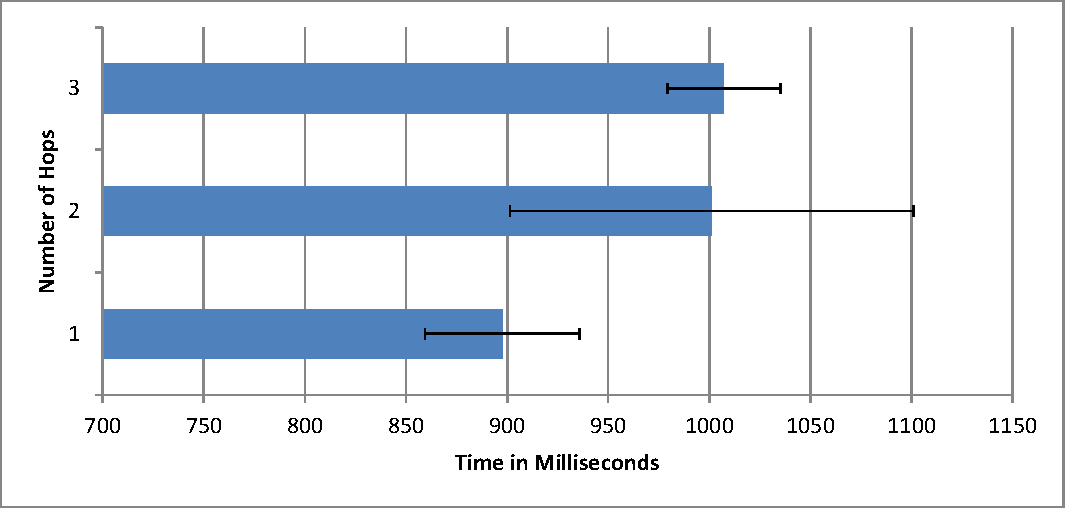
\includegraphics[scale=.65]{graph1.pdf}
\caption{Performance of Identity Token Fetching with 95\% Confidence Interval}
\end{center}
\end{figure}

The values in Figure 3 were obtained over an average of 10 requests. As can be seen, the difference is nearly nonexistent and can be attributed to network variance. These tests were performed with 3 Trust Servers in extremely close proximity, so the results are skewed somewhat. However, these numbers are still enough to see that the majority of the time spent fetching the identity token seems to be somewhat constant and tied to the single signature performed by the destination Trust Server.

Other computations that are performed by the phone are also completed fairly quickly, as illustrated in Figure 4.

\begin{figure}[h]
\begin{center}
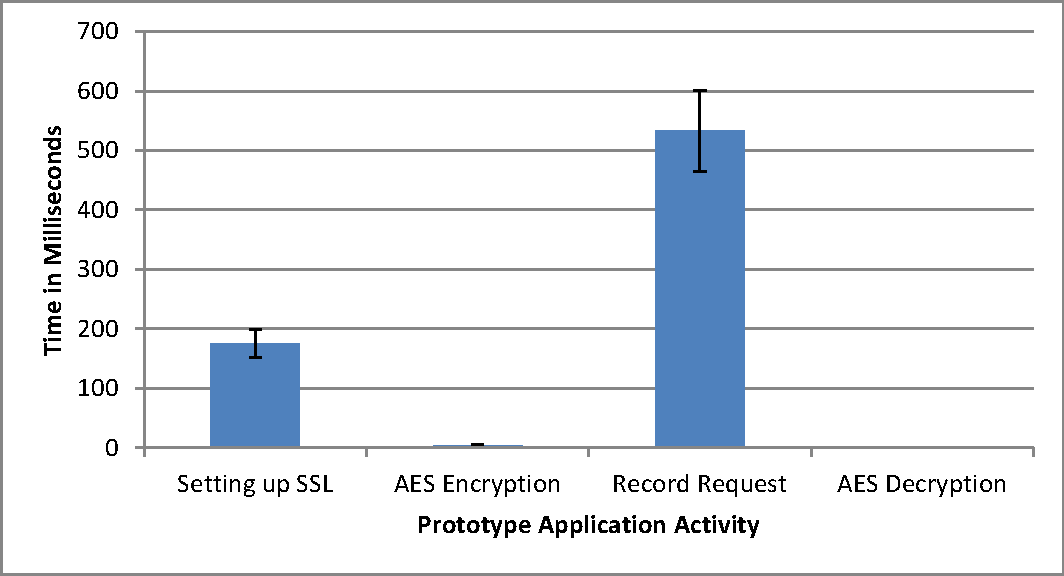
\includegraphics[scale=.65]{graph2.pdf}
\caption{Prototype Performance in Various Tasks with 95\% Confidence Interval}
\end{center}
\end{figure}

Concerns that the encryption/decryption of the health record requests would be too taxing for the phone's processor are quickly laid to rest. The largest bottleneck to performance seems to be the round trip delivery of the health records over the 3G network. This network call does not increase in complexity regardless of health record location, so this time is fairly constant and acceptable in performance.

The prototype seems fairly secure from a security standpoint. All communication is encrypted. There is room for the strengthening in the cryptographic techniques used, but should the appropriate precautions be taken, all communication can be considered reasonably secure. Considering the speed with which this is accomplished, the protocol seems like a reasonable success.
\section{Conclusion}
As shown in Figures 3 and 4, smartphone processors have evolved enough that the encryption steps in this protocol are fairly trivial in terms of time taken. Even the X.509 certificate validation used in SSL completes fairly quickly, and the bandwidth consumed over the network calls is trivial for such small Java objects. The largest concern is in regards to scalability --- not many Trust Server hops were tested while executing the prototype due to infrastructure constrains. A countrywide deployment of the protocol would likely require many more Trust Server hops and take much longer to locate the correct Trust Server responsible for signing the identity token. This could be mitigated by increasing the number of neighbors each Trust Server begins with, although this may become prohibitively expensive to set up.

There are still weaknesses in the protocol that were made apparent during development of the prototype that need to be addressed before it is truly viable for real world usage (these weaknesses will be discussed further in the next section). Even once these weaknesses are addressed, a protocol responsible for such sensitive information as health records should have the utmost security. The proposed protocol would have to be examined much more closely to even begin consideration for use in the wild.

Even assuming the protocol has impenetrable security (an impossible feat), the myriad of regulations it would need to meet to become official likely prevent its use. Still, the successes (and failures) during development serve as a valuable lesson to be used when making protocols of this nature, and serve as a good starting point for future works.
\section{Future Work}
There are a few places the current protocol needs refinement before extensions are considered. First, the method in which Trust Servers locate the patient that is being requested in not clearly defined. In the prototype, this issue is avoided and left up to future implementations to handle. It is assumed that each Trust Server is able to easily look up whether a patient is located in the Health Record Server(s) that the Trust Server is responsible for. Beyond this, something similar to the routing algorithms used in network routers may prove effective. Initial searches during setup may prove time consuming, but if each Trust Server is able to maintain a table of patients and paths through which this patient can be reached, the time cost should stabilize after enough queries. This also has the added benefit of allowing Trust Servers and Health Record Servers to be added to the system without having to notify and reconfigure the entire infrastructure.

The other point of concern is the symmetric key that is used to encrypt communication between the requester and the Health Record Server. In the prototype, the key generation step is skipped and the same key is used for all communication. Although this measures the costs of encryption and decryption, it is not a secure solution for the long term. There are several options here, and key generation and delivery is a well studied problem. A variant of Diffie-Hellman could be used without adding much complexity to the protocol, as long as one is careful to protect against attacks. Or the already encrypted SSL connections of the Trust Servers could be used to deliver unique keys for each session.

There are also many interesting ideas that could be further research for future work on the protocol (or other protocols entirely). The trust mechanisms could be made more robust so as to handle different roles and access restrictions rather than trusting requesters with full access to health records immediately, as discussed in \cite{6040529}.

There are also a myriad of different cryptographic schemes and delivery methods that could be leveraged throughout the protocol. Rather than relying on the arbitrary restrictions imposed by program implementations, perhaps SIP could be leveraged to negotiate the protocols to be used. However, this would add another point of failure in the protocol by the necessity of introducing SIP servers \cite{sparks2007sip}.
\clearpage
\printbibliography[heading=bibnumbered]
\clearpage
\section{Appendix A}
Below are the .java files used in the implementation of the prototype. These files alone are not enough to compile the prototype from scratch as certain minor things like layouts or manifest files are missing. These and all other files necessary to build the project are present in the source repositories. The repository for the Tomcat portion of the project is located at \url{https://github.com/jorgebv/thesis_tomcat/}. The repository for the Android portion of the project is located at \url{https://github.com/jorgebv/thesis_android/}.

There may appear to be duplicates of certain classes in Appendix A and Appendix B. This is due to minor differences between the versions running on Tomcat server instances, and the versions running on Android hardware. Although some files may contain no changes, all files are included below for the sake of completeness.

The prototype makes use of the Apache HttpComponents library version 4.2.5, which can be found here at the time of writing: \url{http://hc.apache.org/downloads.cgi}. These components are licensed under the Apache License, Version 2.0, a full copy of which can be found here: \url{http://www.apache.org/licenses/LICENSE-2.0.html} as well as within the project source directories.

Many of the files below contain references to a library named ``jorgecastle''. The ``jorgecastle'' library is a minimally modified version of the Bouncy Castle 1.48 release, which can be found here at the time of writing: \url{http://www.bouncycastle.org/latest_releases.html}. All that was changed from the stock Bouncy Castle 1.48 release was the renaming of packages to avoid conflicts with outdated Bouncy Castle versions included in Android, and renaming of the Bouncy Castle provider from ``BC'' to ``JC''. This code is not available due to the large size and trivial nature of the changes. These components are licensed under an adaptation of the MIT X11 License, a full copy of which can be found here: \url{http://www.bouncycastle.org/license.html} as well as within the project source directories.
\renewcommand{\lstlistingname}{Android Class}
\setcounter{lstlisting}{0}
\lstinputlisting[language=java, style=eclipse, caption={AES256Encryptor}]{a_AES256Encryptor.java}

\lstinputlisting[language=java, style=eclipse, caption={CMSSignedDataEncryptor}]{a_CMSSignedDataEncryptor.java}

\lstinputlisting[language=java, style=eclipse, caption={Encryptor}]{a_Encryptor.java}

\lstinputlisting[language=java, style=eclipse, caption={RSAEncryptor}]{a_RSAEncryptor.java}

\lstinputlisting[language=java, style=eclipse, caption={IdentityToken}]{a_IdentityToken.java}

\lstinputlisting[language=java, style=eclipse, caption={MainActivity}]{a_MainActivity.java}

\lstinputlisting[language=java, style=eclipse, caption={SSLClient}]{a_SSLClient.java}

\lstinputlisting[language=java, style=eclipse, caption={ThesisLog}]{a_ThesisLog.java}

\lstinputlisting[language=java, style=eclipse, caption={ThesisTimer}]{a_ThesisTimer.java}
\section{Appendix B}
\renewcommand{\lstlistingname}{Tomcat Class}
\setcounter{lstlisting}{0}
\lstinputlisting[language=java, style=eclipse, caption={HealthRecordServerA}]{t_HealthRecordServerA.java}

\lstinputlisting[language=java, style=eclipse, caption={HealthRecordServerB}]{t_HealthRecordServerB.java}

\lstinputlisting[language=java, style=eclipse, caption={HealthRecordServerC}]{t_HealthRecordServerC.java}

\lstinputlisting[language=java, style=eclipse, caption={TrustServerA}]{t_TrustServerA.java}

\lstinputlisting[language=java, style=eclipse, caption={TrustServerB}]{t_TrustServerB.java}

\lstinputlisting[language=java, style=eclipse, caption={TrustServerC}]{t_TrustServerC.java}

\lstinputlisting[language=java, style=eclipse, caption={AES256Encryptor}]{t_AES256Encryptor.java}

\lstinputlisting[language=java, style=eclipse, caption={CMSSignedDataEncryptor}]{t_CMSSignedDataEncryptor.java}

\lstinputlisting[language=java, style=eclipse, caption={Encryptor}]{t_Encryptor.java}

\lstinputlisting[language=java, style=eclipse, caption={RSAEncryptor}]{t_RSAEncryptor.java}

\lstinputlisting[language=java, style=eclipse, caption={IdentityToken}]{t_IdentityToken.java}

\lstinputlisting[language=java, style=eclipse, caption={SSLClient}]{t_SSLClient.java}
\end{document}
